%-----------------------------------------------%
% Modelo de Plano de Aula com três momentos pedagógicos
%
% Autor: Rodrigo Nascimento (2022-08-12)
%-----------------------------------------------%

\documentclass[
% -- opções da classe memoir --
12pt,				% tamanho da fonte
openright,			% capítulos começam em pág ímpar (insere página vazia caso preciso)
oneside,			% twoside para impressão em verso e anverso. Oposto a oneside
a4paper,			% tamanho do papel. 
% -- opções da classe abntex2 --
chapter=TITLE,		% títulos de capítulos convertidos em letras maiúsculas
%section=TITLE,		% títulos de seções convertidos em letras maiúsculas
%subsection=TITLE,	% títulos de subseções convertidos em letras maiúsculas
%subsubsection=TITLE,% títulos de subsubseções convertidos em letras maiúsculas
% -- opções do pacote babel --
english,			% idioma adicional para hifenização
%	french,				% idioma adicional para hifenização
%	spanish,			% idioma adicional para hifenização
brazil				% o último idioma é o principal do documento
]{abntex2}
\selectlanguage{brazil}
%-----------------------------------------------%
% Informações do DOCUMENTO
%-----------------------------------------------%
\instituicao{Universidade do Estado de Santa Catarina -- UDESC}
\titulo{Estágio Curricular Supervisionado -- IV}
\autor{Rodrigo Nascimento}
\local{Joinville - SC}
\data{\mydate}
\tipotrabalho{Plano de Aula}
\orientador{Prof(a). Dr(a). Ana P. Grimes de Souza}
\coorientador{Prof. Me. Mário Heleno Calegari}
%-----------------------------------------------%
% Para alterar o parâmetros dos comandos orientador
% e coorientador.
%-----------------------------------------------%
% \renewcommand{\orientadorname}{Orientadora:}
\renewcommand{\coorientadorname}{Supervisor:}
%-----------------------------------------------%

\newcommand{\centro}{Centro de Ciências Tecnológicas -- CCT }
\newcommand{\departamento}{Departamento de Física -- DFIS}
\newcommand{\curso}{Licenciatura em Física }
\newcommand{\disciplina}{Estágio Curricular Supervisionado IV-- ESC4003}
\newcommand{\firstkey}{Estágio Supervisionado}
\newcommand{\secondkey}{Ensino de Física}
\newcommand{\thirdkey}{Ensino Médio}


%-----------------------------------------------%

%	Todas as indicações de pacotes e configurações estão no arquivo de estilo
%  chamado texmodel-udesc.sty.
\usepackage{texmodel-udesc}

%-----------------------------------------------%
% Estilo de cabeçalho que só contém o número da 
% página e uma linha
%-----------------------------------------------%
\makepagestyle{cabecalholimpo}
\makeevenhead{cabecalholimpo}{\thepage}{}{} % páginas pares
\makeoddhead{cabecalholimpo}{}{}{\thepage} % páginas ímpares
%\makeheadrule{cabecalholimpo}{\textwidth}{\normalrulethickness} % linha
%-----------------------------------------------%

%-----------------------------------------------%
% HEADER
%-----------------------------------------------%
\begin{document}

\thispagestyle{empty}
\begin{center}
	\begin{minipage}[!]{\linewidth}
		\begin{minipage}[!]{.19\linewidth}
			
\includegraphics[width=\linewidth]{img/logo.png}           
		\end{minipage}
		\begin{minipage}[!]{.8\linewidth}
			\center
			\ABNTEXchapterfont\normalsize\MakeUppercase{\imprimirinstituicao}
			\par
			\vspace*{10pt}                     
			\ABNTEXchapterfont\normalsize\MakeUppercase{\centro}
			\par
			\vspace*{10pt}           
			\ABNTEXchapterfont\normalsize\MakeUppercase{\disciplina}
		\end{minipage}        
	\end{minipage}
	\\ \vspace{0.5cm}
	\rule{\textwidth}{.5pt}   
\end{center}
%-----------------------------------------------%
% Ficha de Identificação
%-----------------------------------------------%
\textual
\begin{center}
	\textbf{Plano de Aula: Vento, Temperatura \& Pressão}
\end{center}
\par\noindent\textbf{Estagiário(a):} \imprimirautor\hfill{}\textbf{Orientadora:} Prof(a). Ana Paula Grimes
\par\noindent\textbf{U.E.:} EEB Giovani P. Faraco\hfill{}\textbf{Supervisor:} Prof. Mário Calegari
\par\noindent\textbf{Série:} 2º Ano\hfill{}\textbf{Turma:} Nº(6)
\par\noindent\textbf{Aula:} 003/004\hfill{}\textbf{Data:} 14/04/2023\hfill{}\textbf{Duração:} $2\times 40\min$
\rule{\textwidth}{.5pt}
%-----------------------------------------------%
% Início do Plano de Aula
%-----------------------------------------------%
\bigskip{}  
\noindent
\begin{center}
	\textbf{Efeitos do Aquecimento Diferencial nas Massas de Ar}
\end{center}
\par\noindent\textbf{Resumo da aula:} Na análise dos fenômenos atmosféricos, a velocidade dos ventos é um fator determinante para a classificação do grau de intensidade destes fenômenos, neste sentido, esta atividade tem por objetivo, investigar qualitativamente a origem das correntes de ar sobre os oceanos, a partir dos efeitos do aquecimento diferencial. Como recurso, utilizar-se-á as falas do professor Pedro Dias - (IAG/USP) no contexto da entrevista assistida na aula passada. 
\par\noindent\textbf{Habilidades BNCC:} EM13CNT102.

\section{Objetivo de Aprendizagem}
\begin{itemize}
	\item Discutir os efeitos da mudança de temperatura na pessão do ar sobre os oceanos;
	\item Perceber o surgimento de correntes de ar como fenômeno decorrente da diferença de pressão \textit{a priori};
	\item Construir qualitativamente a noção de força devido ao gradiente de pressão atmosférica.
\end{itemize}

\medskip{}

\noindent\textbf{Núcleo Conceitual:} \emph{Temperatura; Pressão; Gradiente de Pressão.}
\newpage

\section{Procedimento Didático} 
\noindent\emph{1º Momento:} Investigando as causas dos ventos.
\par\noindent\rule{.3\textwidth}{.5pt}  
\par\noindent\textbf{Tempo previsto:} 20 minutos

\noindent\textbf{Dinâmica:}  Fazer uma breve recapitulação da aula passada destacando os seguinte tópicos vistos:
\begin{enumerate}[label=\alph *)]
		\item Classificação dos fenômenos meteorológicos
		\item Locais de Formação \textit{(Oceanos: Tempestades Tropicais, Ciclones, Furacões/Tufões. Continentes: Tornados)}
		\item Distinção entre Tornados e Ciclones
\end{enumerate}

Focar no fenômeno tema da trilha \textit{(Ciclones)} e iniciar uma discussão com a(s) seguinte(s) questão(ões): \textit{"Como se formam os ventos?/O quê empurra o ar e o faz movimentar-se?/Se fecharmos todas as janelas, portas e frestas desta sala, de que forma podería surgir algum vento em algum momento dentro da sala?"}

Lembrá-los que pela segunda Lei de Newton, não é possível algo alterar o seu estado de movimento sem submeter-se à alguma força, se necessário, escrevê-las no quadro e discutir brevemente suas consequências: 
\begin{align}
	\vec{F} &= \vec{0}\\
	\vec{F} &= m \vec{a}\\
	\vec{F}_{ab} &= -\vec{F}_{ba}
\end{align}

Deixá-los pensar e formular suas hipóteses $[\leq 10\min]$.

Ainda que os alunos se lembrem da fala do professor (ou pesquisem pelos celulares) a resposta à esta pergunta não é trivial, e não espera-se que consigam correlacionar corretamente as causas geradoras dos ventos, sejam eles dos Ciclones, Tornados ou de maneira geral. A fala do professor do IAG/USP deve ser referenciada como uma espécie de dica, sendo ela: 
\begin{itemize}
	\item[-] \textbf{Jornalista:} Como se formam os Ciclones?
	\item[-] \textbf{Prof. Pedro Dias:} Os Ciclones se formam em virtude de uma camada espessa de água quente, acima dos 27\Celsius [...]
\end{itemize}
Retomar a aula tomando as hipóteses dos alunos e escrevendo-as no quadro, encerrar esta parte da aula quando todas as hipóteses estiverem expostas.


\vspace{50pt}
\noindent\emph{2º Momento:} Efeitos da temperatura na pressão do ar 
\par\noindent\rule{.3\textwidth}{.5pt}    
\par\noindent\textbf{Tempo previsto:} 30 minutos


\noindent\textbf{Dinâmica:} Com as hipóteses no quadro, discutir as particularidades de cada uma em conjunto com os alunos, a justificativa de cada hipótese devem ser fornecidas pelos alunos autores. Havendo hipóteses discordantes ou similares, destacar estes pontos buscando estabelecer comum acordo.

A discussão deve convergir para conceitos como o de temperatura, pressão, densidade do ar e etc. A medida que estes conceitos forem aparecendo, o professor deve conduzir a discussão para a relação entre eles. 


\vspace{50pt}
\noindent\emph{3º Momento:} Forças oriundas da diferença de pressão
\par\noindent\rule{.3\textwidth}{.5pt}
\par\noindent\textbf{Tempo previsto:} 25 minutos
\par\noindent\textbf{Dinâmica:} É natural que os alunos sintam dificuldades em estabelecer a relação entre as variáveis termodinâmicas $T$, $P$ e $V$ necessária para descrever os fenômenos atmosféricos aqui em foco, esta dificuldade reside no fato de que a origem da força causadora de deslocamentos de massas de ar, emerge do aquecimento diferencial de massas distintas de ar, originando taxas de expansões verticais igualmente distintas, estas taxas de expansão, por sua vez, resulta em diferentes valores de pressão ao longo da superfíce horizontal, o que por fim, induz o escoamento das massas de ar ao longo da superfície horizontal indo da região de maior pressão para a região de menor pressão, matematicamente, a força de pressão $\vec{F}_{gp}$ é expressa em termos do gradiente de pressão $p$ e tem direção oposta ao aumento deste gradiente
\begin{align}
	\vec{F}_{gp} &= -V\nabla p
\end{align}
o que de fato foge substancialmente à intuição dos alunos (e de muitos), no entanto, da equação acima, pode-se constatar que a aceleração da massa de ar em deslocamento, é inversamente proporcional à sua densidade
\begin{align}
	\vec{a}_{gp} &= -\frac{1}{\rho}\nabla p
\end{align}
Logo, uma abordagem pela densidade pode ser um pouco mais adequada.

As as seguintes etapas pode ajudar a construir a compreensão do fenômeno de formação dos ventos devido a diferença de pressão e temperatura, sem que haja prejuízos ao formalismo. Estas etapas devem ser conduzidas de forma dialogada com os estudantes

\begin{enumerate}[label=\roman *)]
		\item Desenhar duas colunas de ar no quadro de tamanhos diferentes e se possível de cores diferentes;
		\item Justificar a diferença de tamanhos por expansão/contração térmica;
		\item Salientar que em ambas as colunas existe diferença de pressão entre a base e o topo da coluna, decorrentes do potencial gravitacional;
		\item Atribuir à coluna de ar maior, uma temperatura maior que a coluna de ar menor;
		\item Justificar esta diferença de temperatura, como decorrente do aquecimento de diferentes porções do ar podendo ser ocasionadas pela diferença de temperatura entre os continentes e o oceano por exemplo \textit{(aquecimento diferencial)};
		\item Inicialmente a pressão na base das colunas de ar são sempre iguais pois no início há uma mesma quantidade de ar em ambas as colunas;
		\item A medida que se compara os valores da pressão verticalmente entre as colunas de ar, deve-se encontrar valores de pressões diferentes cada vez mais acentuados, isso em virtude do potencial gravitacional e do aquecimento diferencial:
			\begin{enumerate}[label=\alph *)]
					\item Na coluna de ar maior, os valores de pressão são deslocados vertical para cima do nível de comparação;
					\item Já na coluna de ar menor, este mesmo nível de pressão encontra-se deslocado verticalmente para baixo;
						\begin{figure}[htb!]
							\centering
							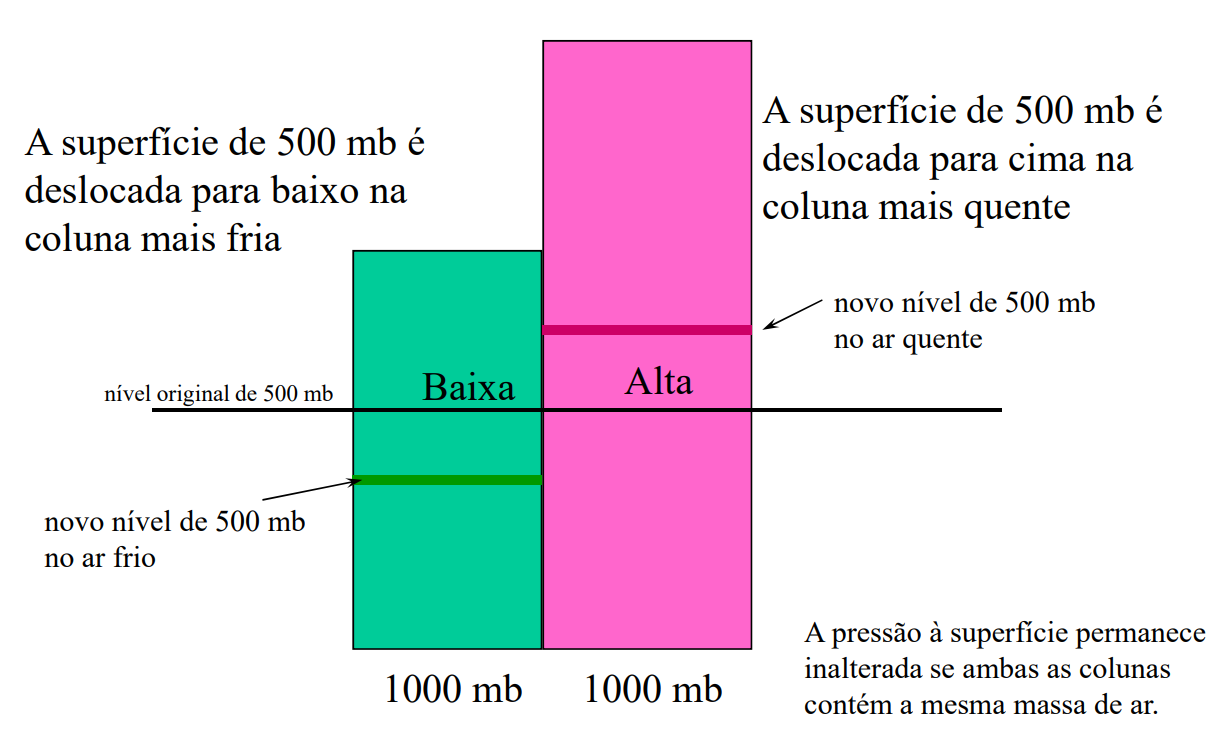
\includegraphics[width=.7\linewidth]{img/deslocamento-ar-01.png}
							\caption{Deslocamento vertical do nível de pressão entre colunas de ar de temperaturas diferentes}
							\label{fig:gradiente01}
						\end{figure}
			\end{enumerate}
		\item Dá-se início á uma corrente de ar entre as duas colunas, com o ar indo da coluna maior para a menor \textit{(Cuidado: Apesar do movimento do ar partir da coluna de maior temperatura, ainda ambas as colunas possuem a mesma quantidade de partículas de ar, portanto na região em que há a migração de partículas esta migração ocorre exclusivamente por diferença de pressão sempre da região onde a pressão é maior para a região onde a pressão é menor)}.
		\item Após a troca de partículas entre as colunas, a pressão na base da coluna de maior temperatura se torna menor, pois agora há menos partículas nesta coluna de ar;
			\begin{figure}[htb!]
				\centering
				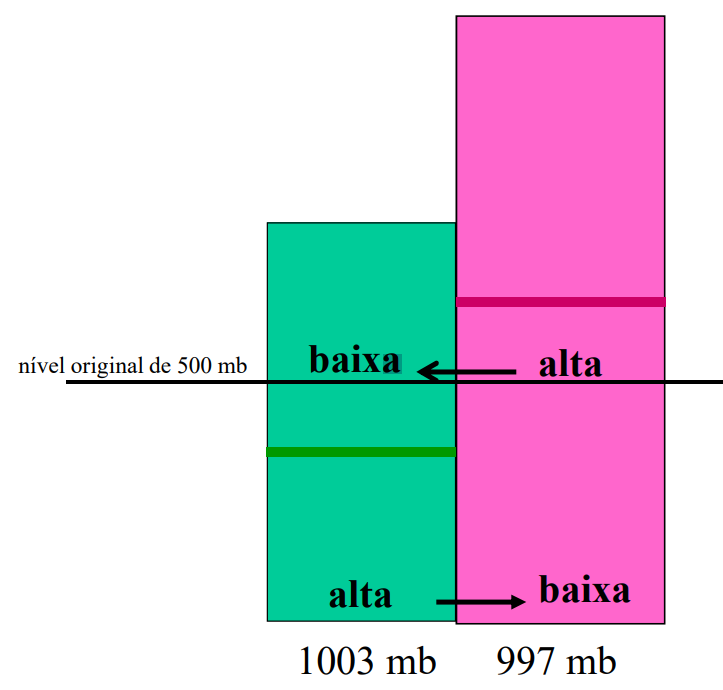
\includegraphics[width=.45\linewidth]{img/deslocamento-ar-02.png}
				\caption{Deslocamento de ar na superfície entre colunas de temperaturas diferentes}
				\label{fig:gradiente02}
			\end{figure}
		\item Como há uma diferença de pressão agora na base das colunas de ar, ocorre uma nova migração do ar nesta região, indo da coluna de maior pressão para a coluna de menor pressão, dando-se origem aos ventos de superfíce.
		\item O processo inteiro se repete, enquanto houver diferença de pressão.
\end{enumerate}

%-----------------------------------------------%
% Referências
%-----------------------------------------------%
% \bibliography{bibliografia.bib}
%-----------------------------------------------%
% Anexos
%-----------------------------------------------%
% \begin{anexosenv}		    
% \end{anexosenv}
%-----------------------------------------------%
% Fim do Plano de Aula
%-----------------------------------------------%
\end{document}
